\chapter{Non-obtrusive detection of emotions}
\label{ch:discussion}

The initial chapters of this thesis presented the theoretical foundations and the work needed to create a novel method for remote detection of emotions of users during the interaction with games. As highlighted by previous research, the understanding of human emotions, as well as the process of automatically detecting them, is the aim of several researchers in a many different fields. As detailed in Chapter \ref{ch:literature-games}, different theories have been proposed to model and study emotions in a variety of contexts, including those related to games. A considerable share of those theories is based on the human physiology, connecting emotional reactions to psychophysiological signals, e.g. HR and facial activity. Several approaches have been proposed to put such models and theories into practice to achieve the ultimate goal of detecting what a person is feeling. Chapters \ref{ch:literature-face} and \ref{ch:literature-physiological}, for instance, describe the connection between emotions and their manifestations in the body, particularly the process of mapping measurable psychophysiological signals into an emotional state.

Emotion detection is a complex and multidisciplinary problem that demands knowledge from many different areas. In this thesis, focus has been given to the field of games research. This chapter presents and discusses the outcomes of this research, which is focused on creating a non-obtrusive method for emotion detection, particularly in the context of games. Results and contributions of this research are aimed at and discussed under the light of games research, however they are likely to be useful for scholars in other fields as well. The following sections also present insights obtained during the systematic investigation and development of the proposed method, including a discussion on how they relate to games research and other areas.

\section{Game-based model for emotion detection}

Commonly the process of detecting emotions using psychophysiological signals relies on mapping the patterns of such signals into an emotional state. As pointed by the literature review conducted in this thesis, a validated way of doing it is by measuring the changes of psychophysiological signals caused by the interaction between users and emotion elicitation materials. Generally the process involves three main parts: emotion elicitation, signal acquisition and the mapping of such signals into an emotional state. Simply put, subjects are exposed to materials that are likely to produce certain emotional reactions, e.g. video and images depicting sad events, followed by observations of how the signals of interest, e.g. HR, change in accordance. Finally the emotion detection is performed by a technique aimed at producing a model to map the changes of those signals into emotional states, e.g. machine learning model like neural networks. The literature review presented in this thesis shows a myriad of different approaches used in each of the previously mentioned parts.

The majority of previous work focuses on producing a group model, where data from several individuals is used to created a trained machine able to detect emotions of any other subject outside the training population. Contrary to the established notion that a group model is better, this research investigated the venue of a user-tailored approach. As pointed by previous findings \parencite{something}, a model trained on data of a given person might be better at predicting the emotional state of such person. This is motivated by the fact that people are different in many aspects, including cultural and personal expectations \parencite{some}. Furthermore it is reasonable to believe that those individual characteristics might be preserved and better accounted for in a method that uses a user-tailored model as opposed to a group model to detect emotions. In this thesis, both the emotion elicitation process and the mapping of psychophysiological signals into emotional states were focused on the notion of the individual as opposed to the group.

\subsection{Calibration games as emotion elicitation}

%When games are used, they are usually gamified version of cognitive tests, or games featuring a well defined difficulty curve, e.g. easy/hard levels. Users have different gaming skills and expectations, so a game designed to be elicitate stresss might not be perceived as such by some users.

%, while previous work explored the use of games as elicitation sources for recognizing user emotions, relying on the emotional states a person can experience \citep{mandryk2006continuous} and which physiological signals are better predictors of such states \citep{jerritta2011physiological},

Previous works have used several different emotion elicitation materials, mainly images and videos, and less often game-related elements. Those materials, however, lack a more user-tailored approach for studying the variations of signals. When games are used, emotional states such as stress and boredom are often inducted by administering a game with the same particular setup, e.g. high/low difficulty, to all subjects. People respond differently to media according to their personality \parencite{ravaja2004effects}, and they differ in social, learning and play styles \parencite{goldberg1993structure}. A game session labeled as stressful, for instance, assumes that all subjects have the same expectations and behave similarly, which dilutes the individuality of each person as some might experience the interaction as not being stressful as intended. Additionally the analysis usually involves the interaction of subjects with some game levels (from the same game) featuring a constant difficulty scale, which does not contemplate the variations of signals in a context where the game difficulty is constantly increasing in the same game level/session.

Investigation of better game-based emotion elicitation materials was one of the main aspects of this research. Aiming to properly elicitate particular emotional states on each user, this research introduced the novel idea of calibration games. As detailed in Section \ref{sec:experiment1-games-elicitation} (on page \pageref{sec:experiment1-games-elicitation}), calibration games are carefully designed and developed games that have a difficulty level that constantly and linearly progresses over time without a pre-defined stopping point. At the beginning the games are highly predictive, without novelties, changes or surprises and with emphasis on the passage of time during a wait, which leads to an emotional state of boredom \parencite{van2010behave,koster2013theory,schell2014art}. The game difficulty is then periodically increased until the subject is not able to cope with the challenges at hand, which happens at different times for different users. The ever-growing game difficulty leads to an emotional state of stress towards the end of the interaction, accounting for the different expectations and gaming skill of a wide range of users.

Sections \ref{sec:experiment1-study1} and \ref{sec:experiment1-study2} presented a detailed analysis regarding how responses of psychophysiological activity, i.e. HR and facial actions (FA), relate to emotional states in a context featuring calibration games. Results show that a calibration game is a valid emotion elicitation material which accounts for personal differences among subjects when inducing emotional states of stress and boredom. Using the proposed calibration games, it was possible to observe and confirm with statistical significance variations of HR and naked-eye recognizable FA that happened during the interactions with the games, especially under situations that were designed to provoke boredom and stress. Those findings were an essential part of the user-tailored method proposed in this thesis, since they proved that calibration games can be used as emotion elicitation material. Another important factor is the nature of the calibration games when compared to other emotional stimuli, e.g. images or videos. The use of images, videos or text as content to produce the emotional stimuli is less likely to produce the reactions of a real gaming session. In a game, users are in charge of actions, which are bound to have consequences. A bad judgment might cause the main character to get hurt, or a right movement might produce a reward. This feedback loop is happening constantly in a game, likely producing emotional reactions on the user. It is plausible to believe that the calibration games present a more sophisticated interaction through their game mechanics, as opposed to the simplistic, one-way interaction between users and images/videos, for instance. Consequentially the use of calibration games is likely to create a deeper emotional connection between users and the emotion elicitation material, resulting in clear and observable changes in psychophysiological signals.

\subsection{Remote readings of psychophysiological signals}

Several of the works found in the literature rely on physical sensors to acquire the signals used in the emotion detection model. Physical sensors are not convenient since they require a cumbersome setup and might disturb the user experience, i.e. invalidate the use of a finger or hand. Use of remote sensing to acquire psychophysiological signals, a non-obtrusive approach of data collection, is mentioned in the literature as a promising solution for that problem. Remote sensing of psychophysiological signals is an essential part of this research, since its objective is to create a method able to non-obtrusively detect user emotions. A complete non-obtrusive method for signal acquisition, however, is a complex and challenging problem, particularly in a context involving games. The literature review conducted for this thesis found the main psychophysiological signals that can be remotely acquired and whose data can be used to detect emotional states.

One of those signals that are commonly acquired using remote and non-obtrusive approaches is facial activity. Chapter \ref{ch:literature-face} (on page \pageref{ch:literature-face}) described in details techniques for facial analysis and the approaches using them for emotion detection. As mentioned in the chapter, results indicate that facial analysis is a promising source of information to be used in the process of emotion detection. Additionally  the combined use of facial and body features (multimodal emotion recognition) is known to perform better than using either one alone \parencite{zacharatos2014automatic}. Following the findings of previous work, the present thesis used facial activity as an important signal in the emotion detection process. A novel method for automated analysis of facial cues from videos was developed, as explained in Section \ref{s:experiment1-study4} (on page \pageref{s:experiment1-study4}). Empirical results of such method show its potential for detecting stress and boredom of players in games. The method is based on Euclidean distances between automatically detected facial points, designed to be robust enough to correctly perform facial analysis even when users are naturaly interacting with games. In such case, players behave naturally as they play, e.g. moving, laughing and speaking. Evaluations of the method were performed experimentally using game-based emotion elicitation, which properly contextualized the efficiency of the method in the field of games research. Results, detailed in Section \ref{s:experiment1-study4}, confirm the method has the potential to differentiate emotional states of boredom and stress of players. However the natural behavior of users during the interaction with the games is a significant factor impacting the process.

%. Secondly we present the results of an automated facial analysis performed on subjects of our experiment, who interacted with different games under boring and stressful gameplay conditions. Our results show that values of facial features detected during boring periods of gameplay are different from values of the same facial features detected during stressful periods of gameplay. Even though the nature of our games, i.e. 2D and casual, and the sample size (N=20) could be limiting factors for the generality of the evaluation of our method, we believe our population of experimental subjects is diverse and our results are still promising. Our study contributes with results that can guide further investigation regarding emotions and facial analysis in gaming contexts. .

Another signal acquired using remote and non-obtrusive approaches is HR and its derivatives. Chapter \ref{ch:literature-rppg} (on page \pageref{ch:literature-rppg}) detailed the progress that has been made in the remote estimation of physiological signals, particularly the use of rPPG to estimate HR. Despite the potential rPPG has to eliminate physical sensors completely, its use is considerably impacted by the natural behavior of users. As presented in Section \ref{s:experiment1-study3} (one page \pageref{s:experiment1-study3}), rPPG estimations of HR are sensitive to noise caused by movement, facial expressions or changes in illumination (e.g. screen activity reflected on user's face), which are all likely to happen in gaming sessions. Those interferences might produce unreliable measurements of the HR signal, resulting in misleading data. Despite those limitations, the use of remote measurement of physiological signals, such as rPPG, has already been applied to emotion detection. Signals as HR and HRV were used to remotely detect stress \parencite{mcduffcogcam, mcduff2014improvements, bousefsaf2013remote}, for instance. In the majority of the cases, subjects are typically instructed to stay still \parencite{rouast2016remote}, which improves the accuracy of the rPPG technique. In some other cases, however, authors evaluate the accuracy of the HR estimation under scenarios where subjects are instructed to act naturally. Despite the fact that such works present experiments where subjects are told to behave naturally, their accuracy evaluation is based on artificial or simple human-computer interactions. Subjects are idly staring at the camera \parencite{zhao2013remote,hsu2014learning}, faking an interaction with a computer \parencite{poh2010non}, working on a task, i.e. make a website \parencite{monkaresi2014machine} or mentally subtract numbers \parencite{mcduff2014remote}, or performing arbitrary movements \parencite{tran2015robust}, e.g. head rotation in different degrees. Differently from previous works, this thesis employed rPPG in a context where users are naturally interacting with games. Information related to HR is an important physiological indication of the emotional state of users, so the use of rPPG was essential in this thesis to remotely acquire HR data. Extensive evaluations were conducted to establish the reliability of remote HR measurements under situations with natural behavior, where users were not instructed to behave differently than what they usually do. Analysis of the accuracy of remote HR estimations clearly established the limitations of the rPPG technique, showing how it is affected by user behavior. One of those identified limitations is the effect that facial occlusion has on the rPPG estimations of the HR. The act of resting the chin on the palm of the hand, for instance, a common trait of bored users, significantly affects the process of detecting a face in the videos, thus directly affecting the estimations of HR. Evaluation results of the rPPG technique, as detailed in Section \ref{s:experiment1-study3}, have shown an average estimation error that lies within the range that still allows the identification of HR variations caused by emotion elicitation materials, as detailed in Section \ref{s:experiment1-study2}. It shows that it is feasible to remotely extract HR and facial data from video recordings of users interacting with games. As a consequence, those signals can be acquired non-obtrusively and used to detect the emotional state of users playing games.

%are presented and discussed. The main contribution of this paper is the accuracy evaluation of an established rPPG technique within the context of gaming sessions where users behave naturally instead of following movement constraint rules, e.g. remain still. Our results provide researchers with information related to the reliability of a remote HR measurement technique when applied to contexts where users behave more naturally

%is drastically impacted by noise introduced by the movement of users. Previous research countered this problem by instructing users to stand still during any interaction, or by limiting the complexity of such interactions, e.g. using images/videos as emotion elicitation materials, not games. In the present research, effort has been put to apply rPPG in a context involving users behaving naturally while interacting with games. Results

\subsection{Multifactorial emotion detection}

The literature review supporting this thesis suggests that the mapping of psychophysiological signals into emotional states based on a multifactorial analysis, when more than one signal is used, is more likely to produce accurate results \parencite{kukolja2014comparative}. As detailed in Chapter \ref{ch:literature-multifactorial}, a combination of signals can reduce the interference and noise caused by signal manipulation, enhancing the accuracy of an emotion detector. Early studies mapping psychophysiological signals into emotional states focused on a multimodal analysis, when more than one modality, e.g. ECG and skin conductivity, are used in conjunction. Such approaches use a wide variety of physical sensors to acquire signal data. As previously mentioned, physical sensors are not ideal, so a completely remote-based approach for data acquisition would be of interest.

As mentioned in Chapter \ref{ch:literature-multifactorial}, a few studies focus on remote extraction of different user signals, i.e. HR and blinking rate, from a single source, i.e. video recording. In such case, a single modality is being used, i.e. video, however a set of different signals (factors) is extracted and used in the emotion detection process, i.e. multifactorial analysis. Despite the fact that those studies use non-obtrusive extraction of user signals for emotion detection, they are not using game-focused elicitation materials. The research presented in this thesis used a novel approach to produce a multifactorial analysis, which is non-obtrusive, user-tailored and game-focused. The overall idea, presented in Section \ref{sec:research-aim} (on page \pageref{sec:research-aim}), is to remotely extract signals from a given user playing the calibration games, then use that data to train a user-tailored neural network, i.e. data from a given user is used to train a single neutral network tailored to that given user. Finally the given user, during the interaction with a particular game, i.e. ordinary, non-calibration game, has signals remotely extracted and fed into the previously trained neural network. The neural network outputs the emotional state of that given user in that particular game.

It is important to highlight that such method for emotion detection based on calibration games, remote sensing and a user-tailored multifactorial analysis has not been found in the literature. Furthermore, its feasibility was unknown and the research reported on this thesis reflects the steps taken to validate such method for emotion detection. In that light, studies 1 to 4, detailed in Sections \ref{sec:experiment1-study1} to \ref{s:experiment1-study4}, were conducted to evaluate each component of such novel emotion detection method. They focused on understanding the capabilities and limitations of each component, including their validity in the process, e.g. use of calibration games as emotion elicitation material. Each of those studies contributed to the final assembling of the novel architecture for emotion detection proposed in this thesis. Finally study 5, detailed in Sections \ref{sec:experiment1-study5} (on page \pageref{sec:experiment1-study5}), was a systematic evaluation of the feasibility of the proposed method when detecting emotions of users actually playing games. It was based on the first experiment conducted and it tested a user-tailored neural network trained on data samples from two calibration games of a given subject which was then used to classify samples from a third calibration game of that same subject. The evaluation included the testing of different user signals, such as HR and facial data combined and used separately. The intent of such evaluation was to better understand the benefits of a multifactorial analysis, confirming that it indeed produces better estimations of the emotional state of users. Results suggested that the proposed method was feasible with potential to non-obtrusively detect the emotional state of user on a user-tailored fashion during the interaction with games.

\subsection{Validation}

The previously described evaluation of feasibility of the proposed method conducted in study 5 was limited by the number of games available for analysis, i.e. three, and the reduced number of subjects. Despite those constraints, results of such study suggested the feasibility of a non-obtrusive, game-based and user-tailored emotion detector. In order to test such indications, a final validation of the proposed method was conducted in a second experiment with a larger sample size, as detailed in Chapter \ref{ch:experiment2} (on page \pageref{ch:experiment2}). In the experiment, the previously mentioned calibration games, i.e. Mushroom, Platformer and Tetris, were used as emotion elicitation materials to train a user-tailored model, i.e. neural network. Such model was then used to detect the emotional state of each user during the interaction with a fourth game, i.e. Infinite Mario. Following the expectations suggested by study 5, the proposed method was able to identify the emotional state of subjects with a mean accuracy of 61.6\%. Results confirmed with statistical significance that the proposed method was feasible and performed better than chance-level classification.

When compared to existing works in the literature, the mean classification accuracy of 61.6\% achieved by the proposed method was still below the mean classification accuracy achieved by other affective computing studies, i.e. 77.91\%. A fair comparison of those numbers, however, is not possible. Each study is conducted in particular situations, using different emotion elicitation materials and different training/testing models. As previously mentioned, the method proposed in this thesis is focused on the individual, not on the group, which is a common factor found in the literature. Another important and highly distinctive difference between the present work and existing ones is how data is obtained to train and evaluate the emotion detection model. The method proposed in this thesis uses a completely independent dataset to train the model, which is obtained from natural interactions of users with game-focused elicitation materials, i.e. calibration games. Those games are similar to COTS games, which portrait a more real gaming experience. The evaluation of the method was conducted on the Infinite Mario game, which mimics the existing commercial game Super Mario. Data from such game was never seen by the trained model, yet it was able to classify the emotional state of users. As mentioned previously, the evaluation of classification performance on fresh data is a better measure for how well classifiers generalize \parencite[Chapter 5]{james2013introduction}. Several works focused on emotion detection do not use game-focused materials for training of a model. Commonly they evaluate accuracy by testings samples that are considerably similar to those found in the training dataset, e.g. splitting available data into training and evaluation datasets, which is different from what is presented in this thesis.

It is unlikely that the method presented by this research, featuring several elements performing under significantly challenging situations, could outperform the accuracy achieved by over 33 affective computing studies undertaken since 1993. It is important to emphasize, however, that the systematic evaluation of the method under different studies and experiments repeatedly indicated its feasibility from statistical analysis. Existing limitations of the proposed method prevent its wide use by researcher and companies, however it is an initiative to move away from questionnaires and physical sensors into a non-obtrusive, remote-based solution for evaluation of user emotions.

 %a larger sample size and a non-calibration game.a more challenging setup  able to detect emotional states of stress and boredom in a larger scequally Following the analysis conducted in study 5, it was expected that

 %that the proposed method would still be feasible when used to detect the emotional state of users in a non-calibration.

 %Finally results suggest that a multifactorial, user-tailored model trained on data samples extracted from calibration games is a feasible method to classify emotional states of user during the interaction with games.

%Physiological signals, e.g. HR, are considered reliable sources since they are hard to fake (because of their link to the ANS), differently from facial expressions \parencite{Landowska}, for instance. When combined in the same analysis, however, those signals can complement each other and provide more information about emotional states.

\section{Insights outside games research}

Contributions of this thesis were aimed at the field of games research, however techniques and theories from a variety of fields, e.g. computer vision and psychology, were used in the investigation process. Several of the pieces that compose the proposed method for emotion detection were studied and evaluated separately, which produced insights of their own that could be used outside the field of games research.

One of such insights relates to the exploration of facial activity under stressful and boring situations. As detailed in Section \ref{sec:experiment1-study1} (on page \pageref{sec:experiment1-study1}), observations of facial actions during the interaction with games indicate that a neutral face remains for longer periods of time during boring periods. Additionally, for the context of the experiment presented in this thesis, facial analysis on an individual level produced more information to connect facial activity to stress/boredom. Such analysis was based on an experiment with a particular configuration that allowed a better exploration of how facial activity relates to emotional states of stress and boredom. Results obtained might be used by other scholars or practitioners interested in understanding or exploring the relationship between facial activity and emotions. In that light, the present research also introduced a novel method for automated analysis of facial behavior, which has been proved to have the potential to differentiate emotional states of boredom and stress of users in real-time. Evaluation of the proposed automated facial analysis show that values of facial features detected during boring periods are different from values of the same facial features detected during stressful periods. Those results can guide further investigations regarding emotions and automated facial analysis. They could also be used as indicators of the emotional state of users in human-computer or human-robot interactions, for instance.

%This paper presented the description and results of an experiment aimed at exploring the variations of heart rate (HR) and facial actions (FA) during gaming sessions with induced boredom and stress. In total twenty adults of different ages and gaming experiences participated in the experiment, where they played three different games while being recorded by a video camera and monitored by a HR sensor. The games used in the experiment were carefully designed and implemented to have a difficulty level that linearly increases over time, from a boring to a stressful point. According to self-reported answers in post-games questionnaires, participants perceived the games as being boring at the beginning and stressful at the end.

%In the context where the measurement of physiological signals by physical and contact-based sensors is intrusive or not desired, e.g. remote estimation of HR, information from different channels is required. One of such additional channels of information might be facial expressions, such as the FA analysis performed in this paper.  We believe that this paper contributes with information regarding HR and FA in the context of games, which can be combined to create user-tailored models for emotion detection based on different data sources.

Another insight relates to remote estimations of HR using rPPG in a context involving natural behavior. The use of rPPG is a promising technique to obtain physiological signals from users/subjects non-obtrusively. Such information has applications in research and the industry. As detailed in Section \ref{s:experiment1-study3} (on page \pageref{s:experiment1-study3}), the evaluation conducted on this thesis regarding rPPG and natural behavior provided more information related to the reliability of remote HR measurements. Even though the evaluation was performed in a context involving games, the analysis still indicates the limitations of the rPPG technique when applied on users interacting with a computer. As demonstrated, user's natural behavior, e.g. movement, affects rPPG estimations to different extents. Such information can guide the use of rPPG in contexts where the mentioned natural behavior is an inherent factor.

Finally this thesis presented an extensive analysis of how physiological signals, particularly HR, relate to emotional states of boredom and stress. As detailed in Section \ref{sec:experiment1-study2} (on page \pageref{sec:experiment1-study2}), this research presented indications that the average HR mean during periods of stress was greater than the average HR mean during periods of boredom in the interaction with games. Similarly to the facial exploration mentioned early, the analysis of the HR activity was performed in an experiment that permitted a more elaborated observation of such activity in boring and stressful interactions. Results of such analysis suggest that changes in the HR is a promising indicator of stress, which contributes information to the body of knowledge of physiological reactions and emotions.

\section{Limitations}

Here I will connect my research with its practical use. I will try to show how it can be used as a tool to enhance the use of questionnaires in game research. I could say that this approach can be used to replace questionnaires, but our numbers do not allow such a bold statement at the moment.


%\begin{figure}[h]
%    \centering
%    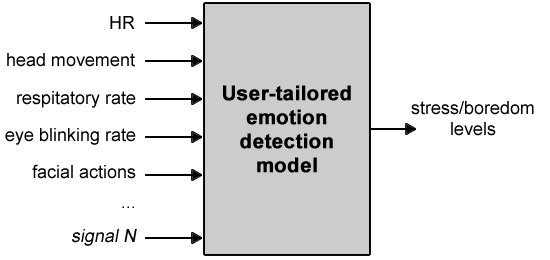
\includegraphics[width=0.6\textwidth]{figures/model-inputs-set.png}
%    \caption{Overall structure of the user-tailored emotion detection model regarding input (user signals) and output (stress/boredom levels).}
%    \label{fig:model-inputs-set}
%\end{figure}

%The user-tailored model proposed for this research might have $N$ input signals, varying from physiological ones, e.g. HR, to non-physiological ones, e.g. facial actions and head movements. Figure \ref{fig:model-inputs-set} illustrates the overall structure of the model. In order to be used in the model, an input signal needs to be supported by previous work regarding emotion detection, as well as be validated within the process of the proposed game-based calibration phase. Time and scope constraints limit the amount of input signals that can be implemented, evaluated and used in this research. As a consequence, a study will be conducted to investigate, validate and initially implement two of those signals into the proposed model: HR and facial activity (which includes head movement, lips activity, etc).

%The techniques and works presented in chapter \ref{ch:literature-face}, which relate to face detection and emotion estimation, suggest that facial analysis is an important component of a multifactorial emotion detection model. Empirical analysis of the data from the first experiment also suggest that individualities regarding facial activities do exist and could be used to estimate emotional states on a user-tailored basis \parencite{bevilacqua2016variations}. As described in section \ref{ch:literature-face-emotion-detection}, facial actions, head movement, lips/eye/mouth activity and distance measurements of detected facial landmarks are viable and proven sources of information for emotion detection.

%Regarding physiological signals, results indicate that the average HR mean for players during the last minute of gameplay is greater than the average HR mean during the second minute of gameplay (chapter \ref{ch:experiment1}, section \ref{s:experiment1-study3}). The findings are aligned with and reinforce previous research that indicates higher HR mean during stressful situations in a gaming context. The findings also suggest that changes in the HR during gaming sessions is a promising indicator of stress.

%The study will involve the definition of how those two signals will be used as inputs for the model. Facial actions, for instance, will probably be detected and measured by the euclidian distance of the facial landmarks. A vector containing the distances will be evaluated as the input for the model. Regarding the HR, its mean and standard deviation during a particular analysis window will be evaluated as input for the model. A software for the detection of those two signals will be created and used to analyse the video recordings of the first experiment (chapter \ref{ch:experiment1}). The inclusion or exclusion of a component of a signal, e.g. variations of the distances of the lips landmark points, will be based on the accuracy to detect them and the frequency they appear in boring and stressful part of the calibration games.
